\documentclass[a4paper,11pt,oneside,openany]{ioniothesis}



\usepackage[dvips]{graphicx}
\usepackage{makeidx}
\usepackage[greek, english]{babel}
%\usepackage[iso-8859-7]{inputenc}
\usepackage{fontspec}
\setmainfont{Arial}
\setmonofont{Courier New}
\usepackage{amssymb}
\usepackage{amsfonts}
\usepackage{color}
\usepackage{ioniostyle}
\usepackage{xcolor}
\usepackage{listings}
\usepackage{enumitem}

\selectlanguage{greek}


\def\tl{\textlatin}
\def\tg{\textgreek}


 
\parindent=0pt

\makeindex
\evensidemargin=0 cm
\oddsidemargin=1 cm
\textwidth=15 cm







% Define custom colors
\definecolor{codebg}{RGB}{240,240,240}
\definecolor{termfg}{RGB}{0,255,255}
\definecolor{termcodebg}{RGB}{40,42,54}



% Define code listing style for C++
\lstdefinestyle{cppstyle}{
    backgroundcolor=\color{codebg},
    basicstyle=\footnotesize\ttfamily,
    keywordstyle=\color{blue},
    stringstyle=\color{red},
    commentstyle=\color{green!50!black},
    morecomment=[l][\color{magenta}]{\#}
}





\newtheorem{theo}{Θεώρημα}[chapter]
\newtheorem{define}{Ορισμός}[chapter]
\newtheorem{collary}{Πόρισμα}[chapter]
\newtheorem{algorithm}{Αλγόριθμος}[chapter]
\newtheorem{example}{Παράδειγμα}[chapter]




%The following line is for one and half spacing
%\linespread{1.3}
%The following line is for double spacing
%\linespread{1.6}

\linespread{1.5}

\usepackage{drop}


\begin{document}




\author{\textbf{Κωνσταντίνος Τουρτσάκης, Π2019140} \\ \textbf{Επιβλέπων:}  -- Μιχαήλ Στεφανιδάκης --}
\title{
\textbf{\LARGE{\textsc{Ιόνιο Πανεπιστήμιο}} 
\bigskip \\
\large{\textsc{Τμήμα Πληροφορικής}}
\bigskip \\ \bigskip \bigskip \bigskip
\bigskip \bigskip 

\includegraphics[width=0.2\textwidth]{./pdffigs/ionio_logo.pdf}
\bigskip \\ \bigskip 
%\texttt{\large{-- Πτυχιακή Εργασία --}}
\texttt{-- Πτυχιακή Εργασία --}
\bigskip \\ \bigskip
\textbf{\Large{\texttt{
Διεπαφή χρήστη διαχείρισης και εκτέλεσης \\
εφαρμογών μέσω πολυτροπικών \\
περιφερειακών συσκευών
}}}
\bigskip \\ \bigskip}
}
\maketitle





\chapter*{}


\begin{center}
\Large{\textbf{Επιβλέπων}}
\end{center}
\prof{Μιχαήλ Στεφανιδάκης}{Αναπληρωτής Καθηγητής}{Ιόνιο Πανεπιστήμιο Τμήμα Πληροφορικής}

\begin{center}
\Large{\textbf{Τριμελής Επιτροπή}}
\end{center}
\prof{Μιχαήλ Στεφανιδάκης}{Αναπληρωτής Καθηγητής}{Ιόνιο Πανεπιστήμιο Τμήμα Πληροφορικής}
\prof{Δημήτριος Ρίγγας}{ΕΔΙΠ}{Ιόνιο Πανεπιστήμιο Τμήμα Πληροφορικής}
\prof{Θεόδωρος Ανδρόνικος}{Αναπληρωτής Καθηγητής}{Ιόνιο Πανεπιστήμιο Τμήμα Πληροφορικής}







  
\pagenumbering{roman}


%Περίληψη
\chapter*{Περίληψη} \pagestyle{headings}





Η χρήση του προσωπικού υπολογιστή έχει παραμείνει η ίδια εδώ και δεκάδες χρόνια.
Σε αντίθεσή όμως με τις εποχές που οι υπολογιστές αποτελούσαν συσκευές που λίγοι
είχαν στη διάθεσή τους, πλέον υπάρχουν σε ένα μεγάλο ποσοστό στα σπίτια των
ανθρώπων. Η χρήση για την οποία προορίζεται επομένως έχει διαφοροποιηθεί και
για αυτόν τον λόγο είναι αναγκαίο να μπορεί ο χρήστης να περιηγηθεί μέσα στο σύστημα
ανάλογα με τις συσκευές εισόδου που ικανοποιούν και αιτιολογούν την χρήση αυτή.
Το πρόγραμμα που αναπτύχθηκε στο πλαίσιο της παρούσας πτυχιακής εργασίας 
προσπαθεί να λύσει αυτό το πρόβλημα, προσθέτοντας λειτουργικότητα
με την οποία ο χρήστης θα μπορεί να περιηγηθεί χρησιμοποιώντας είτε το πληκτρολόγιο,
είτε το ποντίκι είτε ένα χειριστήριο κονσόλας βιντεοπαιχνιδιών. Για την υλοποίηση του
προγράμματος αυτού θα αξιοποιηθεί η βιβλιοθήκη γραφικής διεπαφής Qt, η βιβλιοθήκη
XInput με το οποίο γίνεται διαχείριση εντολών εισόδου χειριστηρίων Xbox και το
σύστημα Windows στο οποίο θα εστιάσει η εφαρμογή. Το Qt είναι μια cross-platform βιβλιοθήκη
για ανάπτυξη εφαρμογών γραφικής διεπαφής και παρέχει οτιδήποτε χρειάζεται μια τέτοιου είδους εφαρμογή. Ο χρήστης κατά την εισαγωγή του
στο πρόγραμμα καλείται να εισάγει το όνομα χρήστη που θα χρησιμοποιήσει η εφαρμογή.
Στην συνέχεια εισέρχεται στο βασικό παράθυρο της εφαρμογής το οποίο αξιοποιείται κυρίως
από το ποντίκι και  το χειριστήριο. Το παράθυρο αυτό έχει 3 καρτέλες. Μία με τις εφαρμογές
του χρήστη, μία με τις αγαπημένες εφαρμογές του χρήστη και μία με τις ρυθμίσεις της εφαρμογής
στην οποία μπορεί να την παραμετροποιήσει . Στις ρυθμίσεις μπορεί επίσης να βρει και ένα
κουμπί για το άνοιγμα του παραθύρου ενός εικονικού πληκτρολογίου στο οποίο έχει πρόσβαση και
μέσω του χειριστηρίου βιντεοπαιχνιδιών. Επιπλέον υπάρχει ένα παράθυρο για την εκτέλεση 
εφαρμογών μέσω του πληκτρολογίου. Αυτό το παράθυρο διευκολύνει την εκτέλεση των εφαρμογών μέσω της
συσκευής αυτής προσθέτοντας λειτουργικότητα περιήγησης και αντιμετωπίζοντας προβλήματα
όπως εστίαση σε λάθος αντικείμενα πάνω στην γραφική διεπαφή. Στον κώδικα της εφαρμογής υπάρχει
μια κλάση στην οποία δημιουργείται η γραφική διεπαφή του προγράμματος αυτού, μια κλάση για την
δημιουργία του εικονικού πληκτρολογίου και μια κλάση για τον έλεγχο εντολών εισόδου από το
χειριστήριο βιντεοπαιχνιδιών. Επιπλέον υπάρχουν συναρτήσεις που "προσομοιώνουν" πατήματα πλήκτρων
και χρησιμεύουν στην αντιστοίχηση των πιέσεων των κουμπιών του χειριστηρίου σε συντομεύσεις που
υπάρχουν στο σύστημα. Τέλος, η εφαρμογή αυτή μπορεί να εγκατασταθεί μέσω ενός installer που έχει
δημιουργηθεί για τον σκοπό αυτό. Ο installer αυτός είναι διαθέσιμος στο αντίστοιχο αποθετήριο που
υπάρχει στο GitHub \footnote{https://github.com/KonstantinosTourtsakis/MultiDev-Launcher/} και περιλαμβάνει τον πηγαίο κώδικα της εργασίας.





\cleardoublepage

%Πρόλογος και Ευχαριστίες
%\chapter*{Πρόλογος και Ευχαριστίες} \pagestyle{headings}
%Η προσπάθεια δημιουργίας ενός προτύπου οδηγιών για τη συγγραφή μιας Πτυχιακής Εργασίας,
τόσο ως προς τη μορφή όσο και ως προς
το περιεχόμενο και τη διάταξη αυτού, ξεκίνησε ιδιαίτερα νωρίς στο 
Τμήμα Πληροφορικής του Ιονίου Πανεπιστημίου.
Ο κύριος σκοπός 
είναι να τεθεί 
με σαφήνεια αλλά και από νωρίς στους φοιτητές τους Τμήματος 
οι δυσκολίες που πρέπει να περάσουν προκειμένου να
τελεσφορήσει επιτυχώς η πτυχιακή τους δοκιμασία 
αλλά και να μη μειωθεί στο ελάχιστο το όποιο αποτέλεσμα
των προσπαθειών τους λόγω απειρίας στη συγγραφή 
επιστημονικών κειμένων υψηλού επιπέδουν όπως είναι
η Πτυχιακή Εργασία.

Η εκπόνηση της Πτυχιακής Εργασίας είναι ουσιαστικά μια δοκιμασία 
όχι μόνο λαμβάνοντας υπόψη τις δυσκολίες 
που συναντά ο φοιτητής αλλά το επίπεδο του αποτελέσματος στο οποίο
θα πρέπει να φτάσει ώστε να θεωρηθεί επιτυχής η προσπάθειά του αυτή.
Η Πτυχιακή Εργασία δεν είναι όπως μια οποιαδήποτε άλλη εργασία, 
αλλά αφού εκπονηθεί θα παραδωθεί στη Βιβλιοθήκη του Τμήματος και θα 
αποτελεί κτήμα γνώσης για τις επόμενες γενιές. Θα είναι
ένα δημόσιο έγγραφο ουσιαστικά στο οποίο όμως θα μπορεί να
έχει πρόσβαση ο καθένας. Εκ τούτου εύλογα προκύπτει πως όχι μόνο
το περιεχόμενο αλλά και η ίδια η μορφή της θα πρέπει να είναι
προσεγμένη, μάλλον αυστηρή, περίκαλλος και σίγουρα να προσάδει
επιστημονοσύνης.

Ο φοιτητής ερχόμενος προς τη δοκιμασία αυτή κατά το τελευταίο έτος
των σπουδών του θα πρέπει να γνωρίζει πως στο πρόσωπο 
του επιβλέποντος καθηγητή του θα βρει έναν
αξιόλογο συμπαραστάτη και συμβουλάτορα.
Η ίδια η διαδικασία απαιτεί συμβουλές και ένα προχωρημένο επίπεδο,
αρκεί να αναλογιστεί
κανείς πως ο βαθμός δεν δίδεται από έναν και μόνο διδάσκοντα αλλά θα
πρέπει να συναινέσει μία τριμελής επιτροπή στην οποία όλα τα
μέλη έχουν την ίδια βαρύτητα ψήφου.
Επίσης, η διαδικασία εξέτασης της Πτυχιακής Εργασίας είναι δημόσια
στη διάρκεια της οποίας ο φοιτητής θα πρέπει να απαντήσει 
πειστικά σε ερωτήσεις και σχόλια.

Τα παραπάνω δεν θα πρέπει να φοβίζουν τους φοιτητές αλλά μάλλον να αποτελούν
πρόκληση για την εκπόνηση πραγματικά αξιόλογων εργασιών.
Η εμπειρία έχει δείξει πως τελικά η εκπόνηση μιας καλής Πτυχιακής Εργασίας,
βοηθάει τους αποφοίτους στα πρώτα επαγγελματικά τους βήματα,
τα οποία είναι ιδιαίτερα σημαντικά για την καριέρα τους.

Το παρόν πρότυπο απέχει μακράν της τελειότητας
αλλά είναι μια πρώτη προσπάθεια να τεθούν 
ορισμένοι κανόνες ώστε η επίπονη προσπάθεια των
φοιτητών κατά τη διάρκεια της Πτυχιακής Εργασίας
να μην απαξιωθεί στο ελάχιστο λόγω ελλιπούς προβολής.
Οποιαδήποτε σχόλια και προτάσεις είναι δεκτά στο \tl{email: okon@ionio.gr} ώστε να
καταφέρουμε οι διδάσκοντες να βελτιώνουμε συν τω χρόνω
το επίπεδο σπουδών του Τμήματός μας. 


Με τις σκέψεις αυτές και με πολλές ευχές
από όλους τους συναδέλφους 
διδάσκοντες του Τμήματος Πληροφορικής
 για καλή επιτυχία στο επίπονο έργο της
Πτυχιακής Εργασίας σας ευχόμαστε Καλό Πτυχίο!!!
\bigskip \\
Κέρκυρα, \today \\
Κωνσταντίνος Τουρτσάκης
 



\cleardoublepage

\tableofcontents
\cleardoublepage




\listoffigures
\cleardoublepage
\listoftables

\setlength{\parskip}{5pt}



\pagestyle{headings}
\cleardoublepage


\newpage
\pagenumbering{arabic}


\cleardoublepage


\chapter{Εισαγωγή} \label{chapter:intro}




\drop{Ε}{ίναι}
πλέον σίγουρο πως η χρήση ενός προσωπικού υπολογιστή γίνεται μέσω του
πληκτρολογίου σε συνδυασμό με την χρήση του ποντικιού για την περιήγηση του
χρήστη μέσα στο γραφικό περιβάλλον των σύγχρονων συστημάτων. Όμως αυτό ήταν
ανέκαθεν μια μέθοδος περιήγησης που προορίζονταν για εργασιακή χρήση. Με την
εξέλιξη των τεχνολογιών και την εισαγωγή ολοένα και περισσότερων πολυμεσικών
εφαρμογών στο περιβάλλον του Η/Υ, ήταν αναπόφευκτη η μετάβαση σε μια εποχή
όπου ο Η/Υ έχει εφαρμογή σε κάθε σπίτι ανεξαρτήτως του επαγγέλματος του
ιδιοκτήτη. Αναγνωρίζοντας την αλλαγή αυτή και το γεγονός πως παραμένουν
περιθώρια βελτίωσης από την πλευρά του συστήματος ώς προς την επικοινωνία
μεταξύ του χρήστη και του υπολογιστή, το πρόγραμμα αυτό έχει ως στόχο την
εκτέλεση εφαρμογών ανεξαρτήτως της συσκευής εισόδου του χρήστη. Επομένως,
απώτερος σκοπός είναι η αξιοποίηση των νέων περιφερειακών συσκευών στην
εκτέλεση και περιήγηση του λειτουργικού συστήματος αλλά και την υλοποίηση
νέων διαδικασιών εκτέλεσης εφαρμογών από προϋπάρχουσες συσκευές, όπως το
πληκτρολόγιο και το ποντίκι. Για την υλοποίηση αυτής της εφαρμογής είναι
απαραίτητο να γίνει χρήση τεχνολογιών για την γραφική διεπαφή χρήστη και την
είσοδο δεδομένων από τις περιφερειακές συσκευές στο σύστημα. Για την
εξυπηρέτηση αυτών των αναγκών γίνεται κυρίως χρήση της βιβλιοθήκης Qt6, του
XInput και της βιβλιοθήκης των Windows.








\chapter{Ανάπτυξη εφαρμογών σε Qt6} \label{chapter:qt6}





%\section{Qt6 Desktop Applications}
\section{Τι είναι το Qt;}
Το Qt είναι μια δημοφιλής βιβλιοθήκη ανάπτυξης εφαρμογών διεπαφής χρήστη το
οποίο είναι διαθέσιμο σε C++ και Python. Με το Qt
είναι εφικτή η υλοποίηση cross-platform εφαρμογών με το τελικό αποτέλεσμα
να είναι μια αξιοπρεπής διεπαφή χρήστη που λειτουργεί αποτελεσματικά και
αξιόπιστα, υποστηρίζοντας μια πληθώρα συστημάτων όπως Windows, Linux, MacOS, Android και ενσωματωμένα συστήματα. 
Παρακάτω γίνεται περιγραφή της λειτουργίας της βιβλιοθήκης αυτής όπου στην 
περίπτωση αυτή θα γίνει χρήση παραδειγμάτων σε γλώσσα προγραμματισμού C++ 
μιας και είναι η γλώσσα στην οποία έχει γραφεί το παρόν πρόγραμμα.

\section{Ένα απλό πρόγραμμα σε Qt6}
Για την δημιουργία ενός παραθύρου Qt6 πρέπει πρώτα να δημιουργηθεί ένα αντικείμενο
τύπου \textbf{QApplication} και στην συνέχεια να αρχικοποιηθεί ένα αντικείμενο 
\textbf{QWidget} το οποίο θα αποτελεί το παράθυρο της εφαρμογής πάνω στο
οποίο θα προστεθούν τα υπόλοιπα στοιχεία της γραφικής διεπαφής για τις λειτουργίες
του προγράμματος. Παρακάτω βλέπουμε ένα παράδειγμα με την αντίστοιχη περιγραφή
μεταφρασμένη σε κώδικα.

\begin{lstlisting}[language=C++, style=cppstyle]
#include <QApplication>
#include <QWidget>


class MyWidget : public QWidget 
{
public:
    MyWidget(QWidget *parent = nullptr) : QWidget(parent) 
    {
        setFixedSize(400, 300);
        setWindowTitle("P2019140 - Konstantinos Tourtsakis");
    }
};

int main(int argc, char *argv[]) 
{
    QApplication app(argc, argv);

    MyWidget widget;
    widget.show();

    return app.exec();
}

\end{lstlisting}

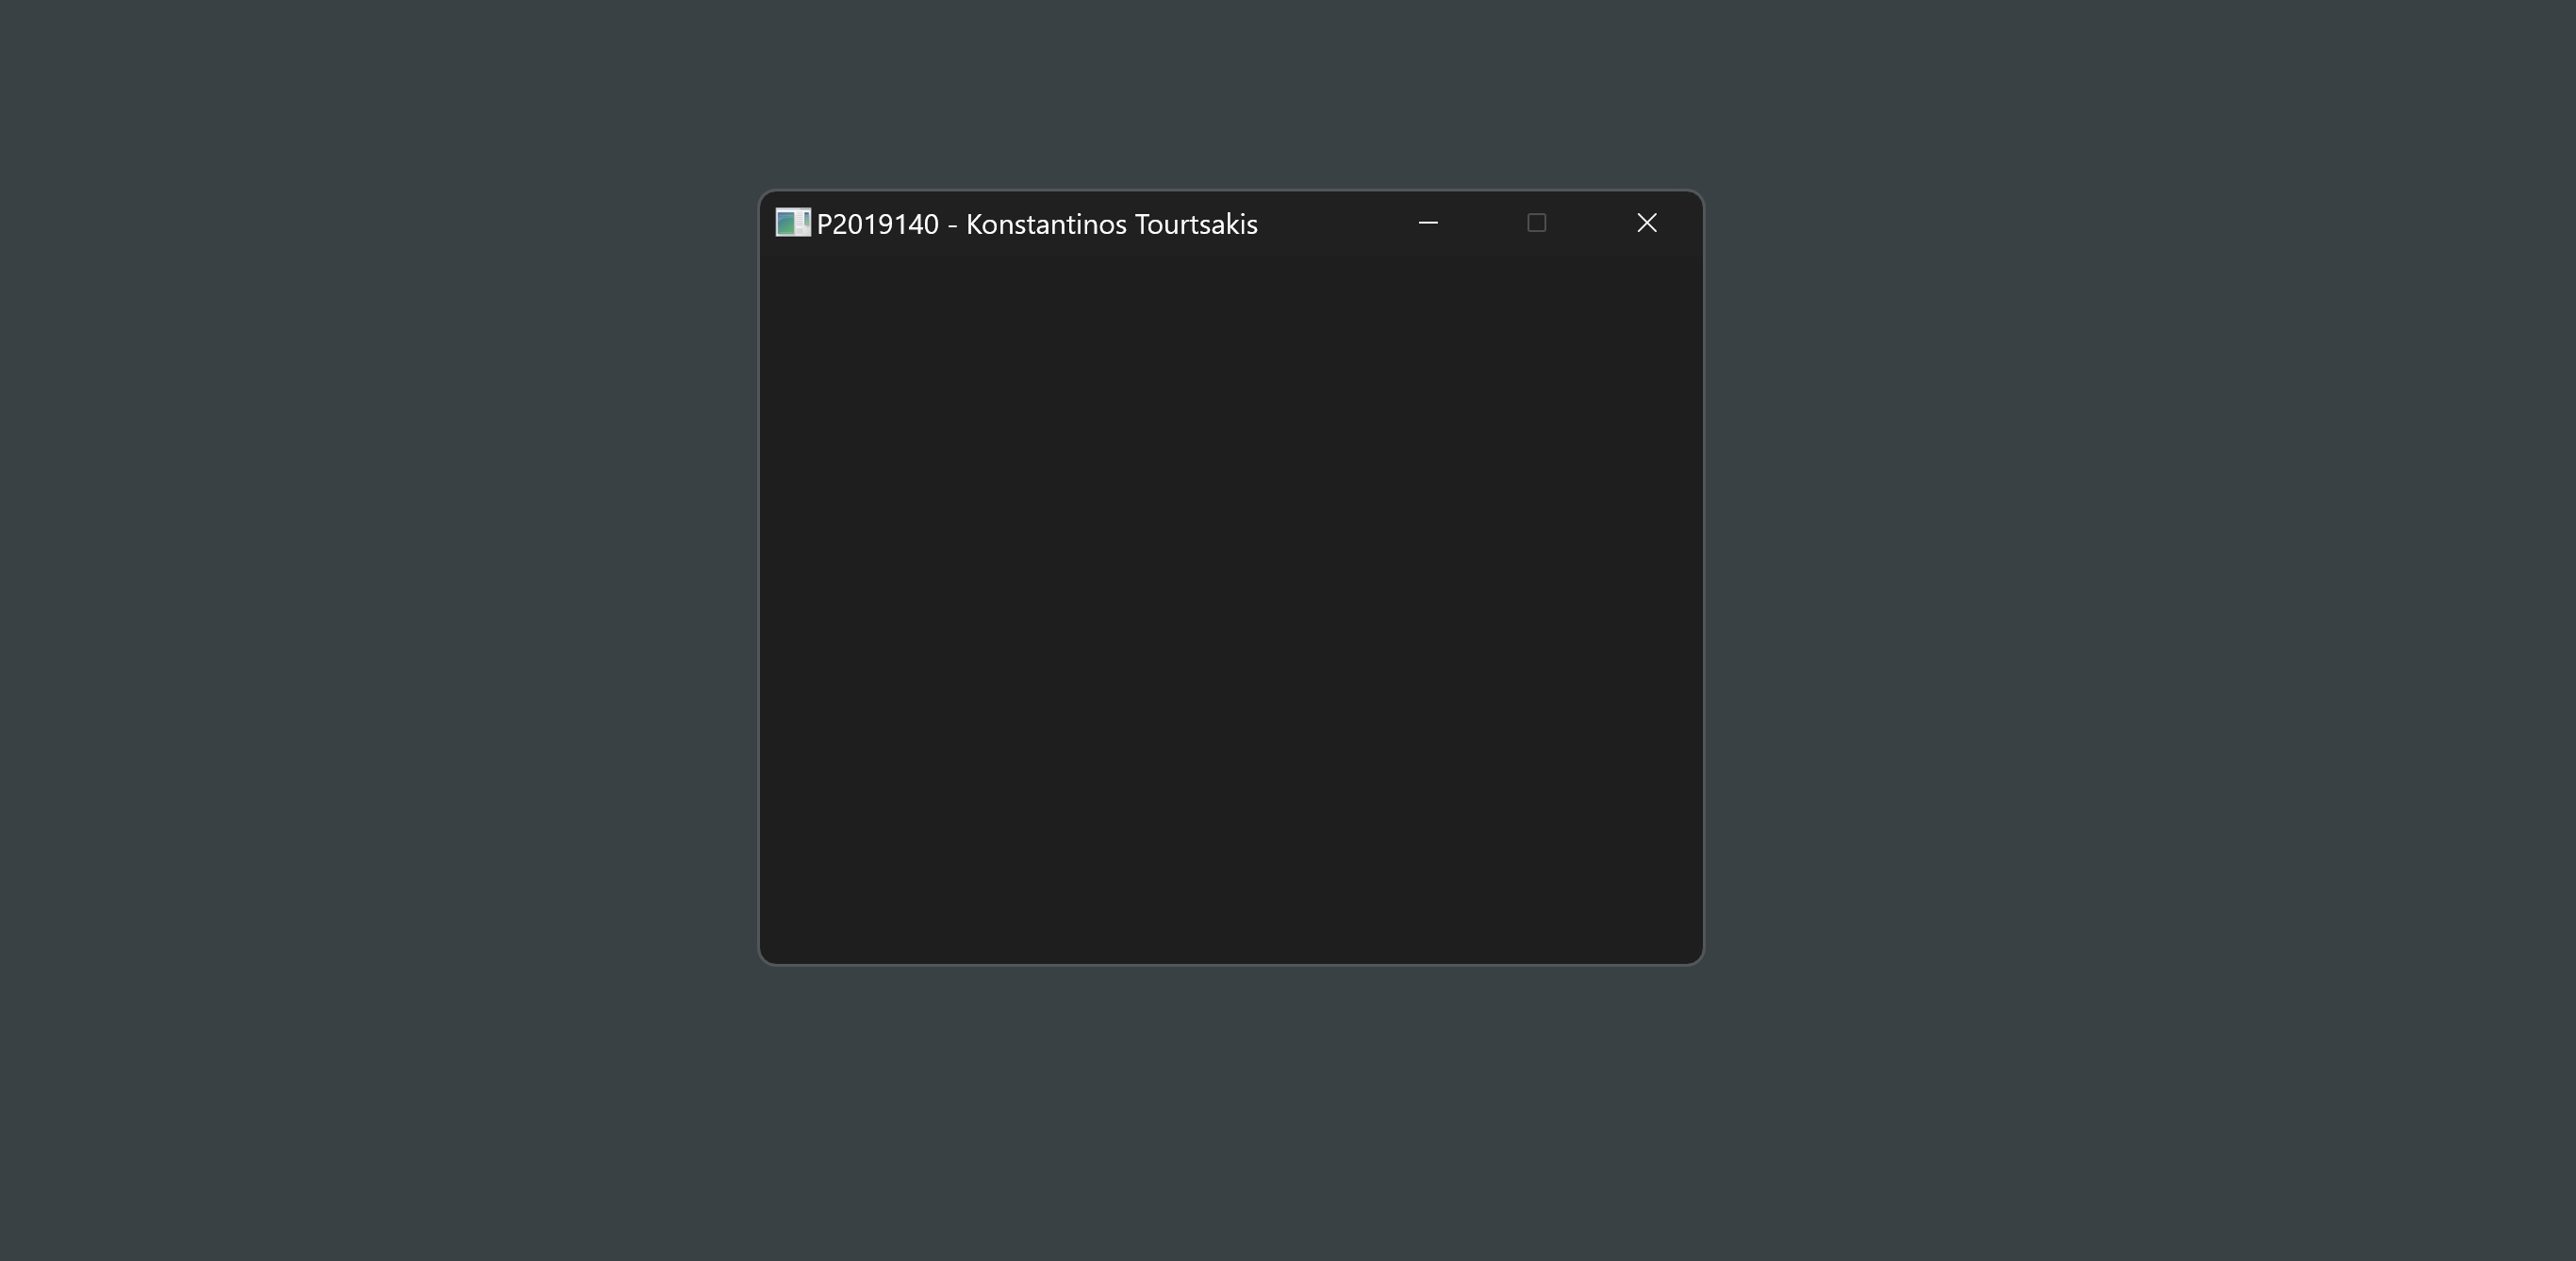
\includegraphics[width=1.0\textwidth]{./images/simple_qt6_app.png}

Η κλάση MyWidget κληρονομεί την κλάση QWidget. Το παράθυρο το οποίο δημιουργείται
εμφανίζεται σε πλήρες μέγεθος και στην συνέχεια επιστρέφεται το αντικείμενο της εφαρμογής
το οποίο το διαχειρίζεται η βιβλιοθήκη κατά την έξοδο εκτέλεσης του προγράμματος.


\section{Προσθήκη στοιχείων γραφικής διεπαφής σε Qt6}
Κάθε εφαρμογή γραφικής διεπαφής παρέχει στοιχεία μέσω των οποίων γίνεται η διαχείριση
των δεδομένων που επεξεργάζεται και η εκτέλεση των λειτουργιών του. Συνήθως τα δεδομένα αυτά δεν είναι τίποτε άλλο από
τους βασικούς τύπους δεδομένων που υποστηρίζουν οι γλώσσες προγραμματισμού:
int, bool, float και string. Επιπλέον υπάρχουν στοιχεία με τα οποία εξυπηρετήται
αποτελεσματικότερα ο σκοπός του προγράμματος, είτε λόγω ευκολίας είτε λόγω κατανόησης
από τον χρήστη. Παρακάτω βλέπουμε τα στοιχεία που αξιποιεί το πρόγραμμα της
εργασίας για την επίτευξη του σκοπού του.

\subsection{Δημιουργία QPushButton}
Ένα QPushButton είναι ένα κουμπί το οποίο έχει την ιδιότητα εκτέλεσης λειτουργιών.
Για την προσθήκη μιας λειτουργίας πάνω στο κουμπί αυτό χρειάζεται να γίνει η
σύνδεση μεταξύ του αντικειμένου αυτού και μιας μεθόδου που ανήκει στην κλάση που
κληρονομεί το QWidget. Ορίζεται το signal το οποίο υποστηρίζει το κάθε αντικείμενο
μέσω του οποίου θα γίνει η κλήση της μεθόδου που ονομάζεται slot από το Qt.
Τα signals που υποστηρίζουν τα στοιχεία του Qt είναι διαφορετικά, ανάλογα με τους
στόχους που προσπαθεί να πετύχει το κάθε ένα από αυτά. Επομένως ένα στοιχείο QPushButton
μπορεί να έχει περισσότερα ή λιγότερα singals σε σύγκριση με ένα QComboBox.
Παρακάτω βλέπουμε ένα παράδειγμα σε κώδικα.
\begin{lstlisting}[language=C++, style=cppstyle]
class MyWidget : public QWidget 
{
public:
    MyWidget(QWidget *parent = nullptr) : QWidget(parent) 
    {
        setFixedSize(300, 200);
        setWindowTitle("P2019140 - Konstantinos Tourtsakis");

        QPushButton *button = new QPushButton("Hello, World", this);
        button->setGeometry(100, 100, 100, 30);

        connect(button, &QPushButton::clicked, this, &MyWidget::PrintHello);
    }

public slots:
    void PrintHello() 
    {
        std::cout << "Hello, World!" << std::endl;
    }
};
\end{lstlisting}

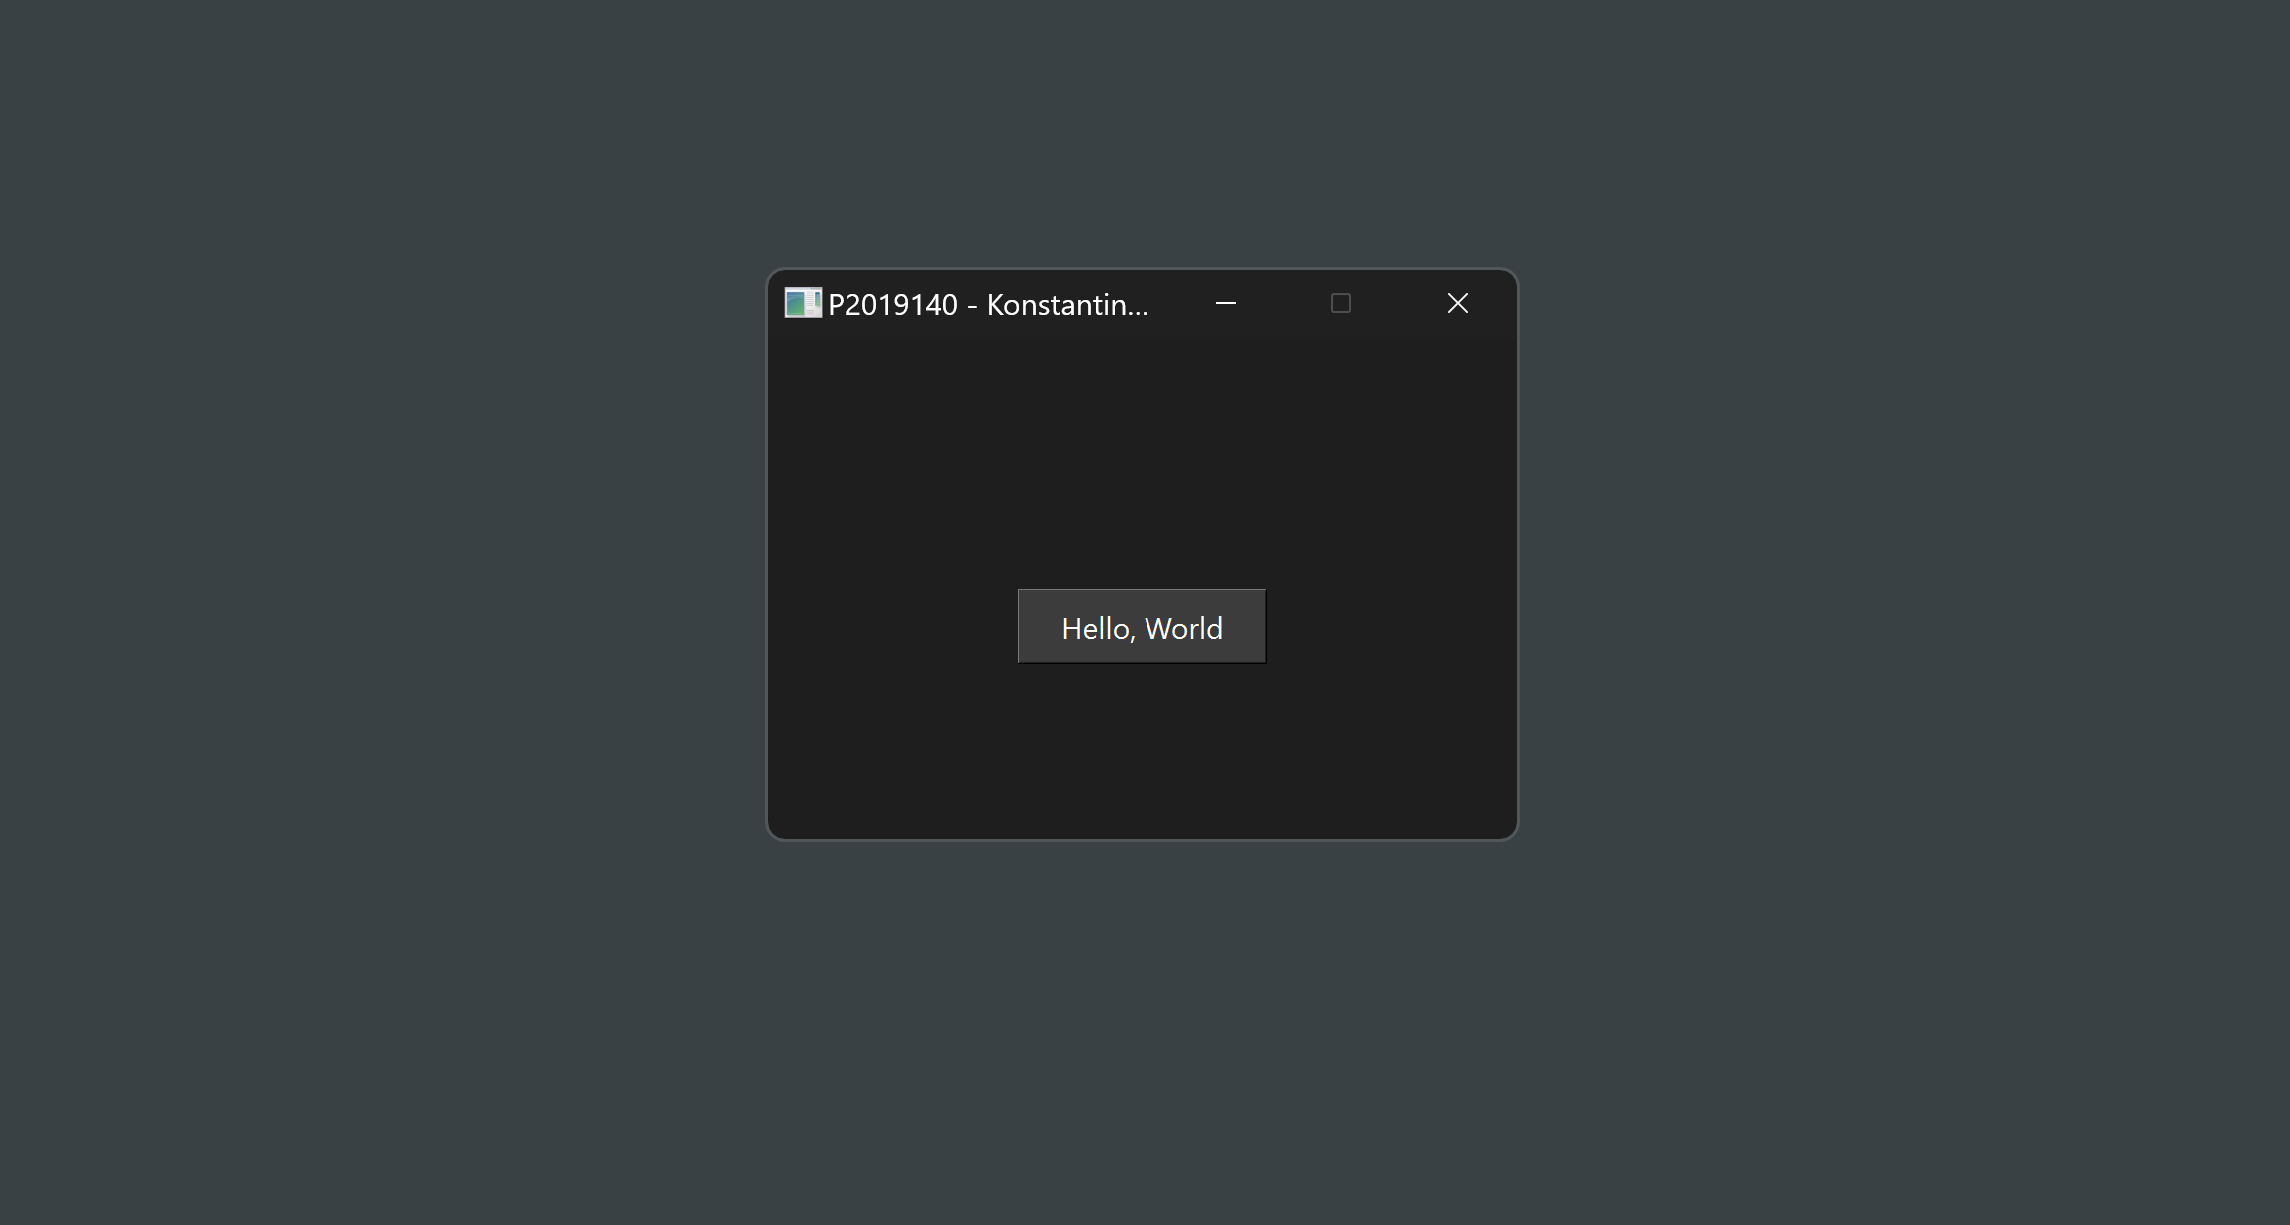
\includegraphics[width=1.0\textwidth]{./images/QPushButton.png}

Στο παράδειγμα γίνεται ή δημιουργία και ή αρχικοποίηση κουμπιού με το όνομά του και στην συνέχεια η σύνδεση.
Στην σύνδεση καλείται η μέθοδος \textbf{connect} στην οποία ορίζεται το signal το οποίο
θα πυροδοτήσει την κλήση του slot που έχει ανατεθεί στο αντικείμενο. Στην προκειμένη περίπτωση έχουμε
ορίσει το QPushButton::clicked signal το οποίο συνδέει το κουμπί με την μέθοδο PrintHello.

\subsection{Δημιουργία γραφικού πλαισίου}
Ένα layout είναι ένα πλαίσιο στο οποίο μπορούν να τοποθετηθούν άλλα στοιχεία του Qt, όπως
το QPushButton που προαναφέρθηκε. Το Qt6 παρέχει 3 βασικά είδη layouts. Το \textbf{QVBoxLayout}, το
\textbf{QHBoxLayout} και το \textbf{QGridLayout}. Τα πρώτα δύο παρέχουν ένα παρόμοιο πλαίσιο με την μόνη
τους διαφορά να βρίσκεται στην κατεύθυνση των στοιχείων μέσα στο πλαίσιο. Επομένως, ένα
QVBoxLayout χρησιμοποιείται για στοιχεία που θα τοποθετηθούν κάθετα (vertical) και ένα
QHBoxLayout θα χρησιμοποιηθεί για στοιχεία που πρόκειται να τοποθετηθούν όριζόντια (horizontal).
Τέλος, ένα QGridLayout χρησιμοποιείται για την τοποθέτηση στοιχείων σε μορφή πίνακα. Το
πλαίσιο αυτό διαθέτει θέσεις που αναπαριστούν ένα σημείο σε έναν δισδιάστατο χώρο. Κάθε σημείο
έχει μια θέση η οποία είναι μοναδική και είναι προσβάσιμη μέσω της τιμής της σειράς και της
στήλης στην οποία βρίσκεται. Παρακάτω βλέπουμε κώδικα με την χρήση ενός QVBoxLayout και την
προσθήκη ενός QPushButton σε αυτό.
\begin{lstlisting}[language=C++, style=cppstyle]
	MyWidget(QWidget *parent = nullptr) : QWidget(parent) 
    {
        setFixedSize(300, 200);
        setWindowTitle("P2019140 - Konstantinos Tourtsakis");
        
        QVBoxLayout *layout = new QVBoxLayout(this);

        QPushButton *button = new QPushButton("Hello, World", this);
        button->setGeometry(100, 100, 100, 30);

        layout->addWidget(button);

        connect(button, &QPushButton::clicked, this, &MyWidget::PrintHello);
    }

\end{lstlisting}

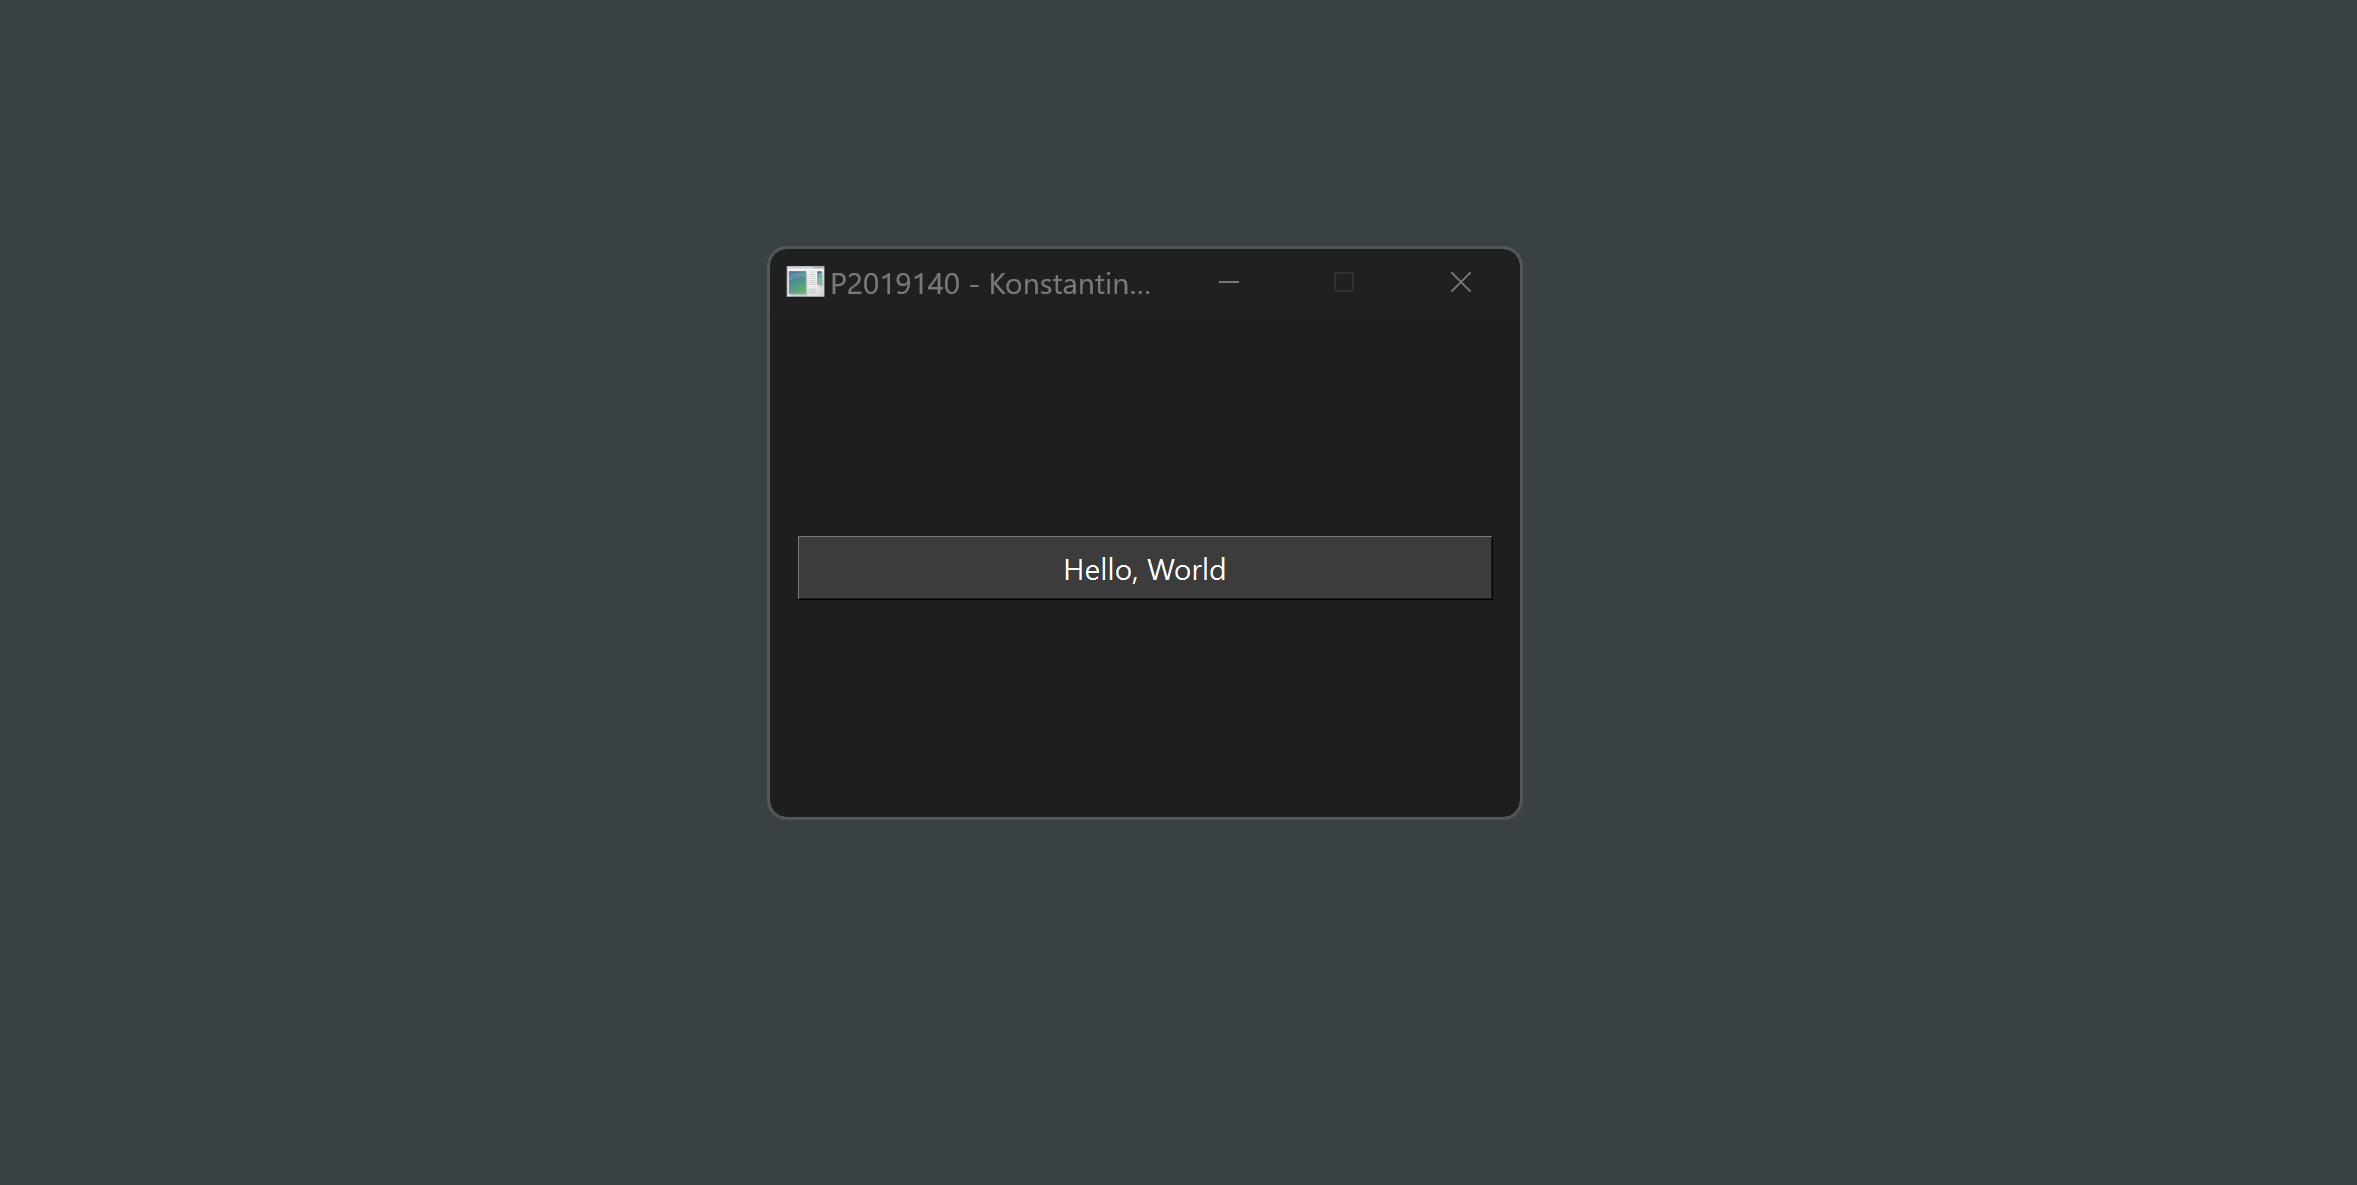
\includegraphics[width=1.0\textwidth]{./images/QVBoxLayout.png}

Κάθε στοιχείο τύπου QWidget προστίθεται πάνω στο layout με την κλήση της μεθόδου
\textbf{addWidget} και αντίστοιχα η αφαίρεση του γίνεται με την μέθοδο \textbf{removeWidget}.

\subsection{Δημιουργία λίστας αντικειμένων}
Μια λίστα QWidget μπορεί να αποθηκεύσει στην μνήμη στοιχεία τύπου QListWidgetItem.
Τα στοιχεία αυτά είναι αντικείμενα του Qt τα οποία δεν μπορούν να αποθηκευθούν σε
κάποια άλλη 


\begin{lstlisting}[language=C++, style=cppstyle]
#include <QListWidget>
#include <QListWidgetItem>


class MyWidget : public QWidget 
{
public:
    MyWidget(QWidget *parent = nullptr) : QWidget(parent) 
    {
        setFixedSize(400, 300);
        setWindowTitle("P2019140 - Konstantinos Tourtsakis");

        QListWidget *list_widget = new QListWidget(this);
        list_widget->addItem(new QListWidgetItem("Item 1"));
        list_widget->addItem(new QListWidgetItem("Item 2"));
        list_widget->addItem(new QListWidgetItem("Item 3"));
        list_widget->addItem(new QListWidgetItem("Item 4"));
        list_widget->addItem(new QListWidgetItem("Item 5"));
        list_widget->setGeometry(10, 10, 200, 200);
    }
};
\end{lstlisting}

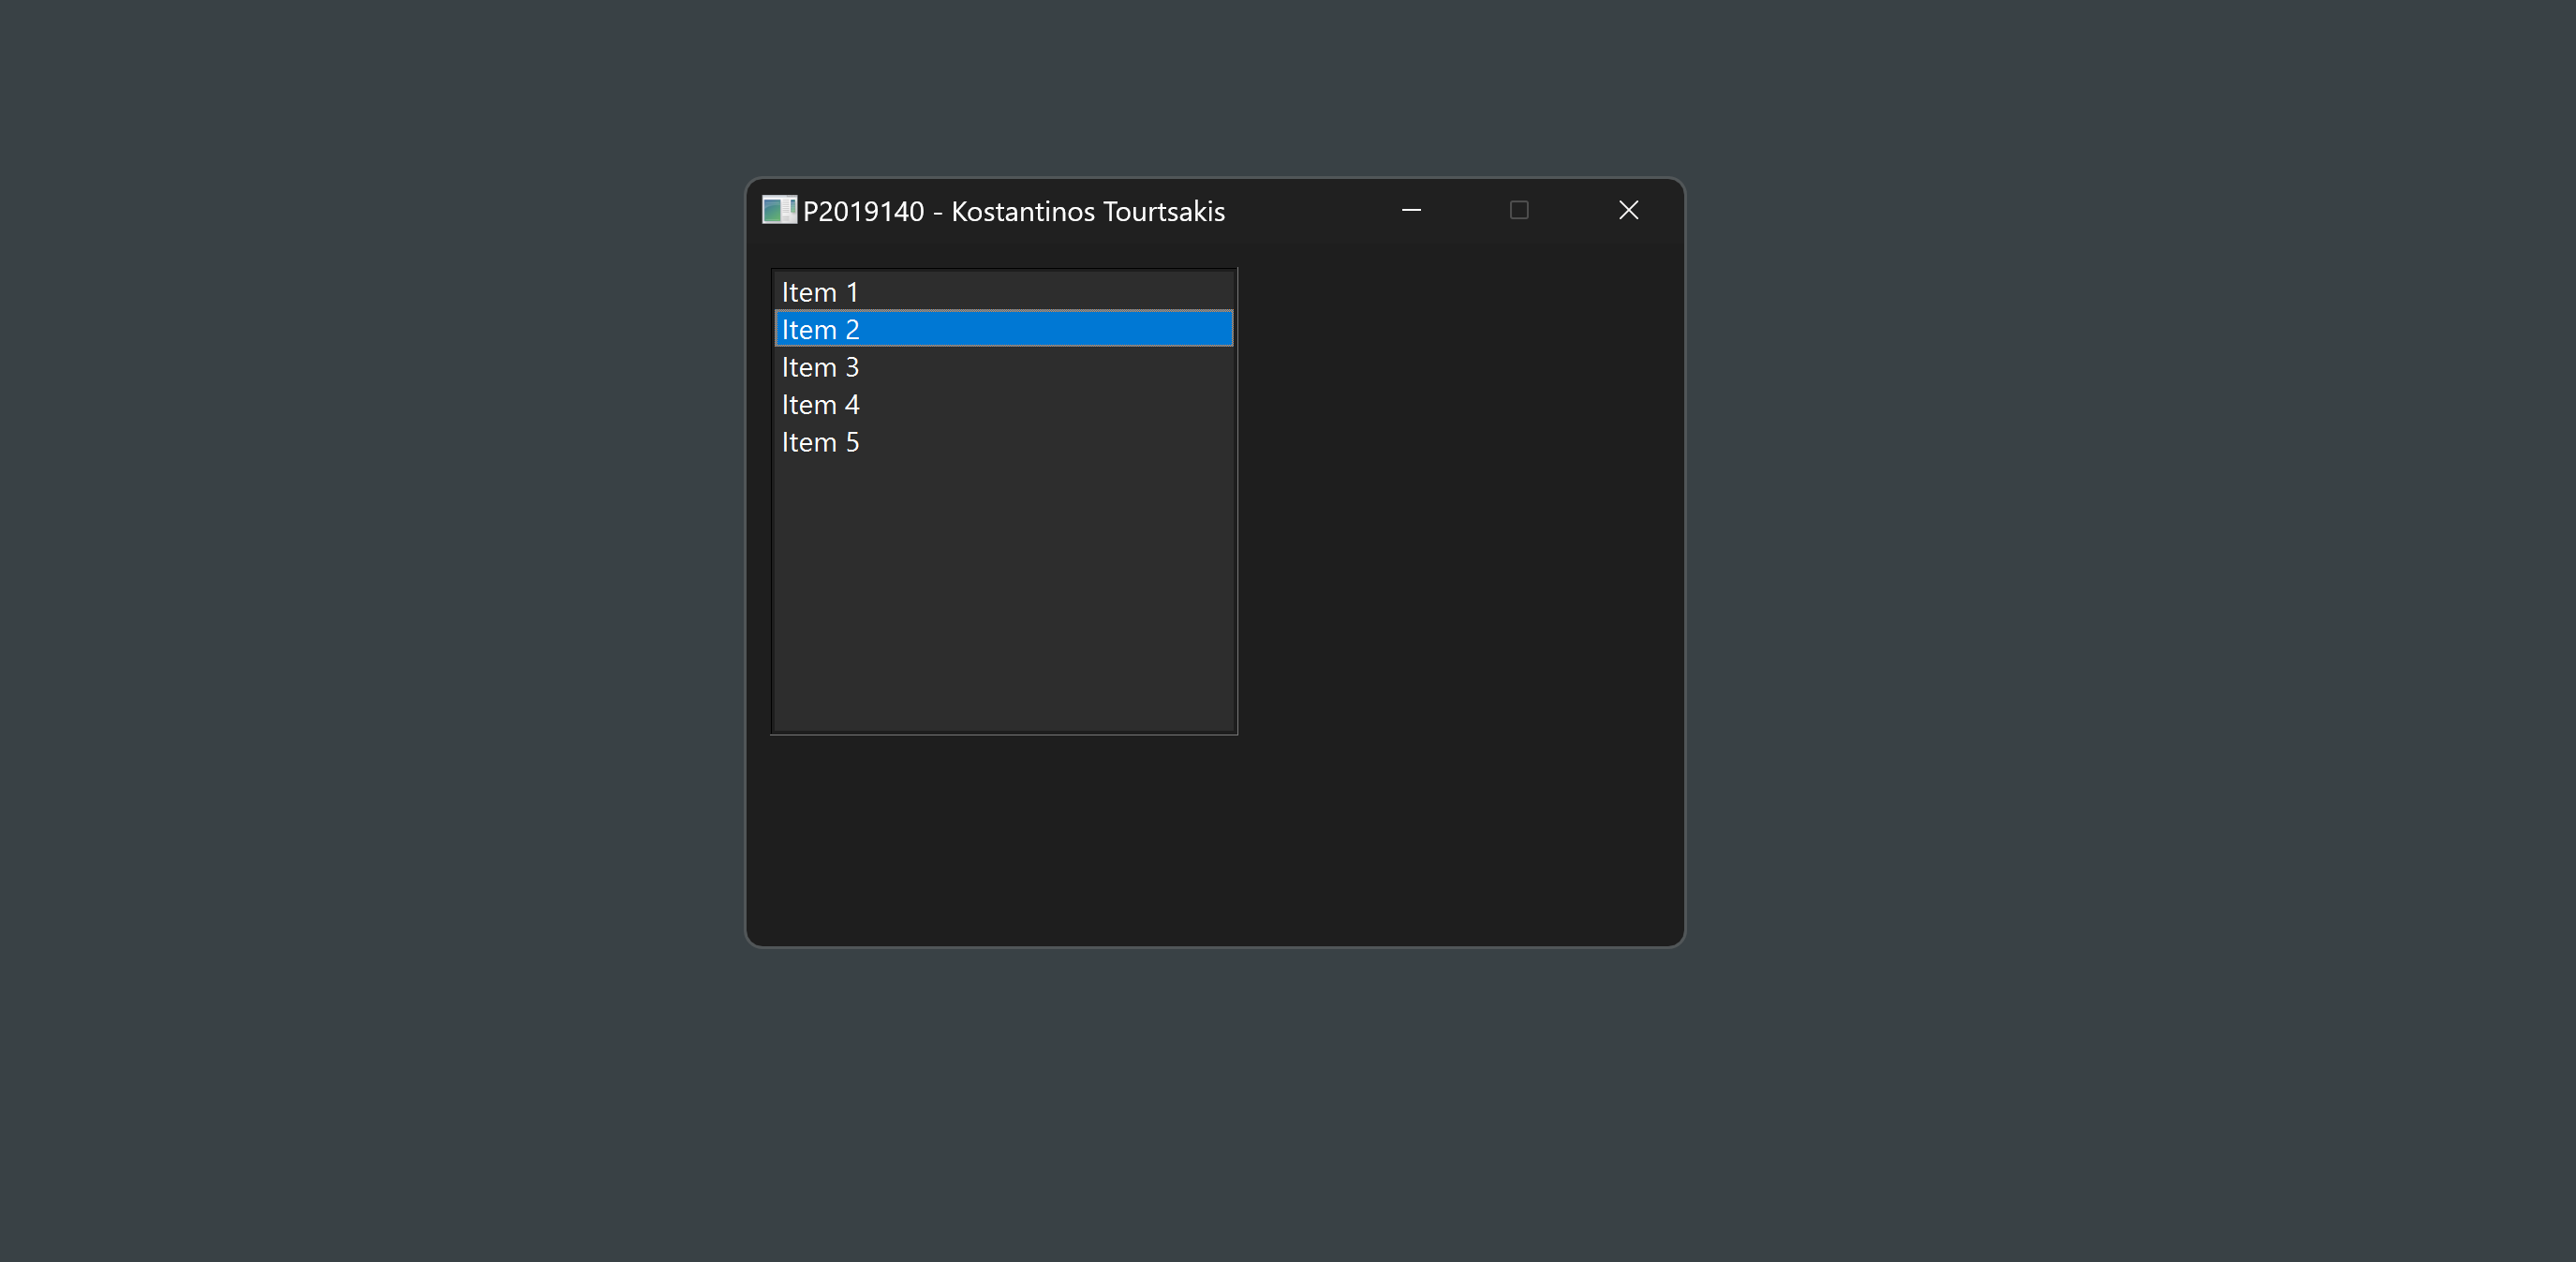
\includegraphics[width=1.0\textwidth]{./images/QListWidget.png}

\subsection{Διάβασμα αρχείων από directory}
Το διάβασμα αρχείων από ένα directory γίνεται μέσω της QDir κλάσης στην οποία
αρχικοποιείται ένα αντικείμενο με το path του directory του οποίου θέλουμε να
διαβάσουμε. Στην συνέχεια αποθηκεύουμε τα αρχεία του directory σε μια λίστα
από QStrings και τα προσπελαύνουμε για την προσθήκη τους σε ένα QListWidget
με στόχο την προβολή τους στον χρήστη.
\begin{lstlisting}[language=C++, style=cppstyle]
#include <QDir>
#include <QStringList>


class MyWidget : public QWidget 
{
public:
    MyWidget(QWidget* parent = nullptr) : QWidget(parent) 
    {
        setFixedSize(300, 200);
        setWindowTitle("P2019140 - Konstantinos Tourtsakis");

        QVBoxLayout* layout = new QVBoxLayout(this);
        QListWidget* list_widget = new QListWidget(this);
        layout->addWidget(listWidget);

        QDir directory("C:\\Users\\kosta\\Documents\\Git\\Thesis\\source\\x64\\Debug");

        QStringList files = directory.entryList(QDir::Files);
        for (const QString& file : files) 
        {
            list_widget->addItem(file);
        }
    }
};
\end{lstlisting}

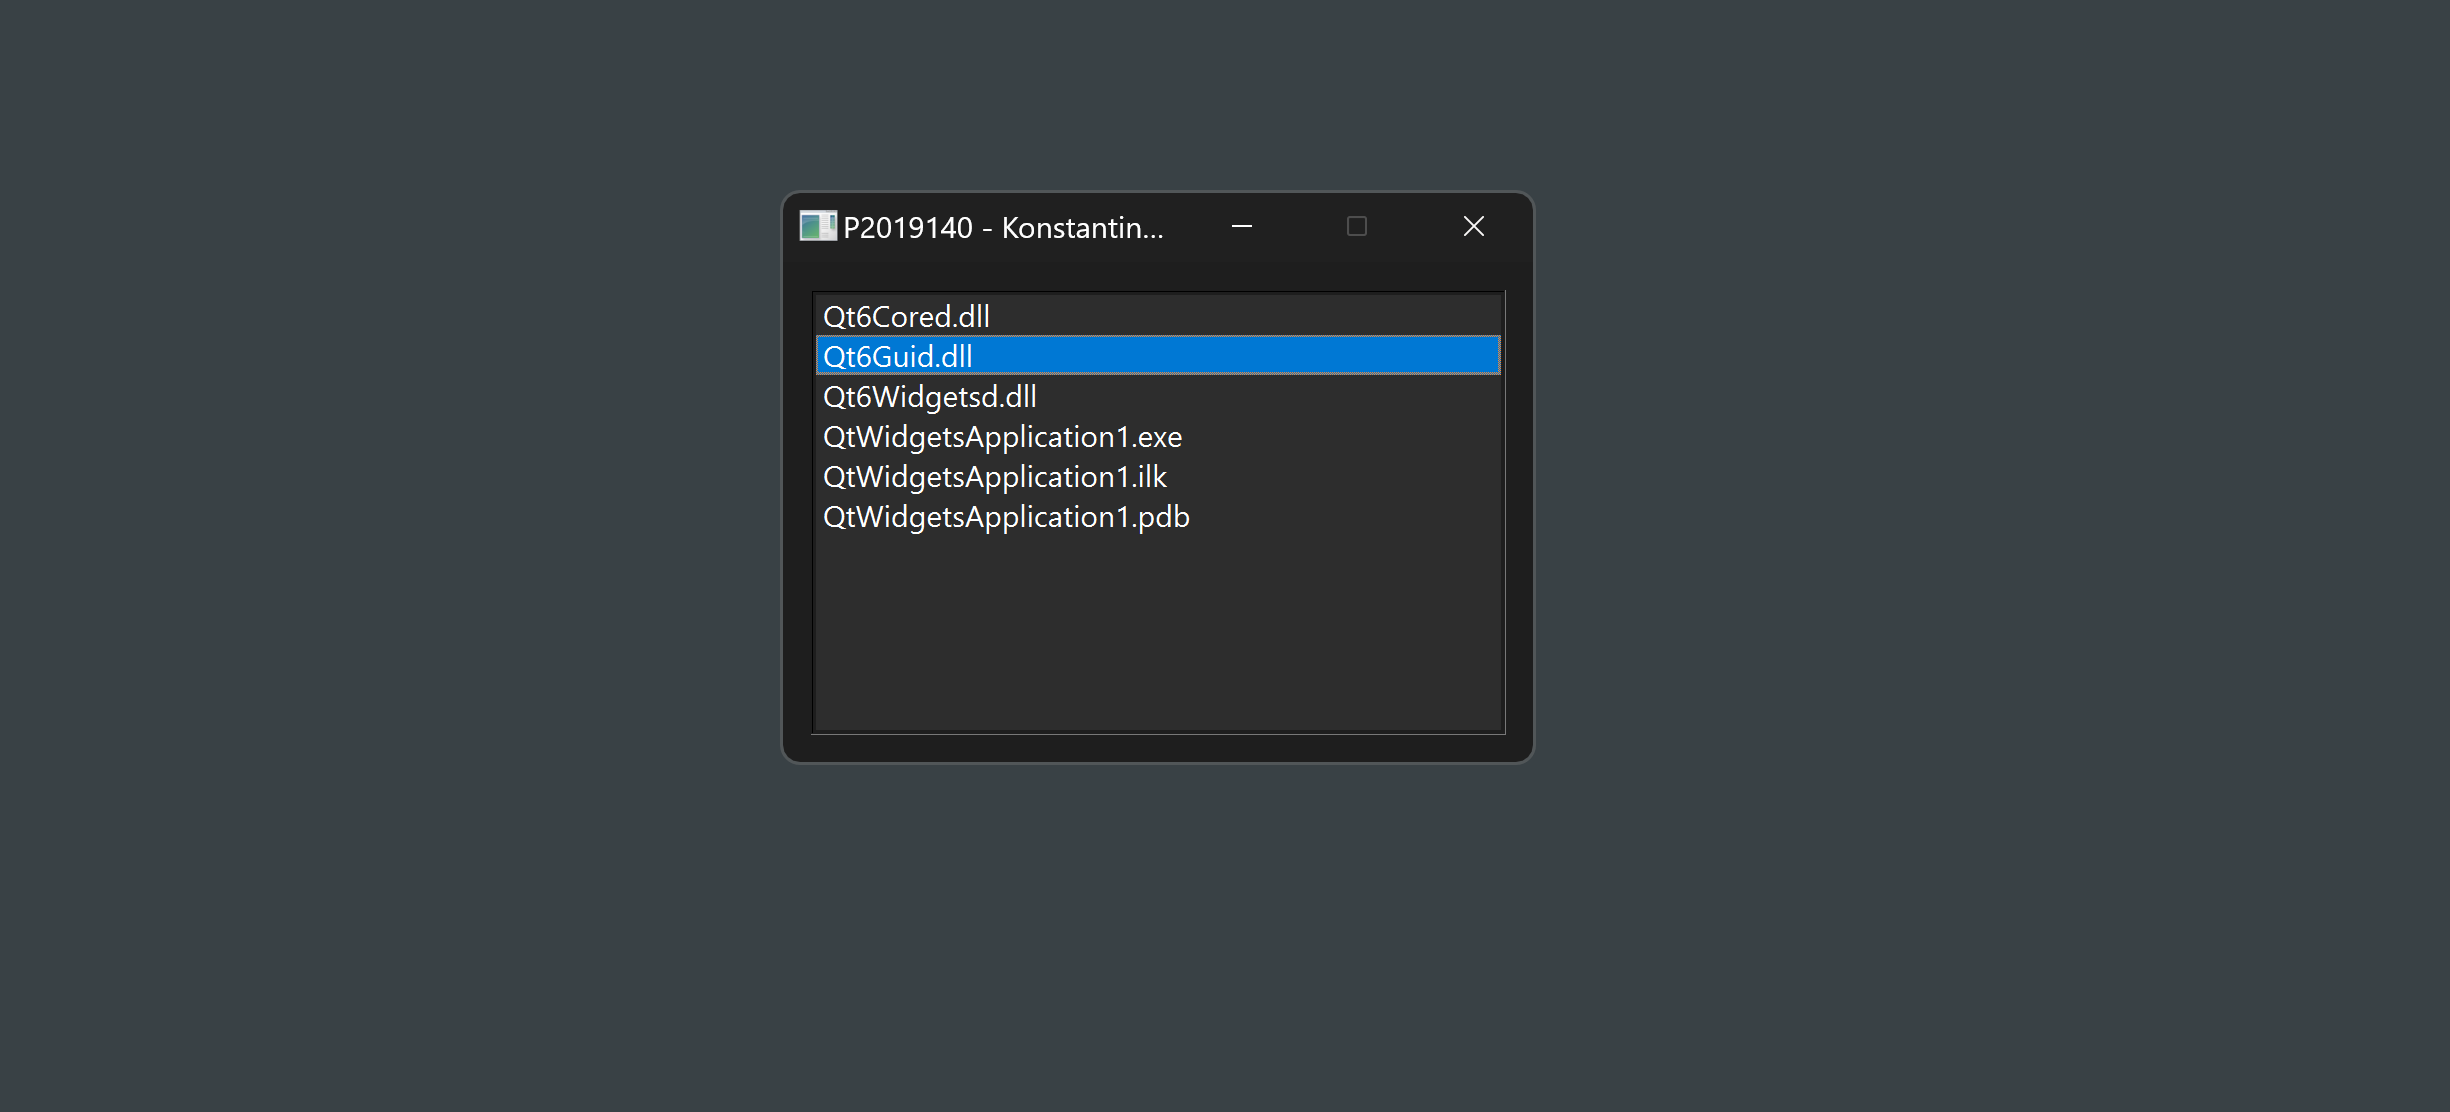
\includegraphics[width=1.0\textwidth]{./images/QDir_file_reading.png}

\subsection{Δημιουργία input field}
Βασικό στοιχείο κάθε εφαρμογής γραφικής διεπαφής αποτελεί ένα input field μιας
και επιτρέπει στον χρήστη να πληκτρολογήσει δεδομένα εισόδου για την εκτέλεση
μιας λειτουργίας του προγράμματος. Για τον σκοπό αυτό το Qt παρέχει τα αντικείμενα
τύπου QLineEdit. Όπως και τα QPushButton, τα αντικείμενα αυτά αρχικοποιούνται
και στην συνέχεια προστίθενται πάνω σε ένα πλαίσιο μέσω της μεθόδου addWidget.


\begin{lstlisting}[language=C++, style=cppstyle]
#include <QLineEdit>

class MyWidget : public QWidget 
{
public:
    MyWidget(QWidget* parent = nullptr) : QWidget(parent) 
    {
        setFixedSize(400, 300);
        setWindowTitle("P2019140 - Konstantinos Tourtsakis");

        QLineEdit* lineEdit = new QLineEdit(this);
        lineEdit->setPlaceholderText("Your input goes here");
        
        QVBoxLayout* layout = new QVBoxLayout(this);
        layout->addWidget(lineEdit);

        setLayout(layout);
    }
};
\end{lstlisting}
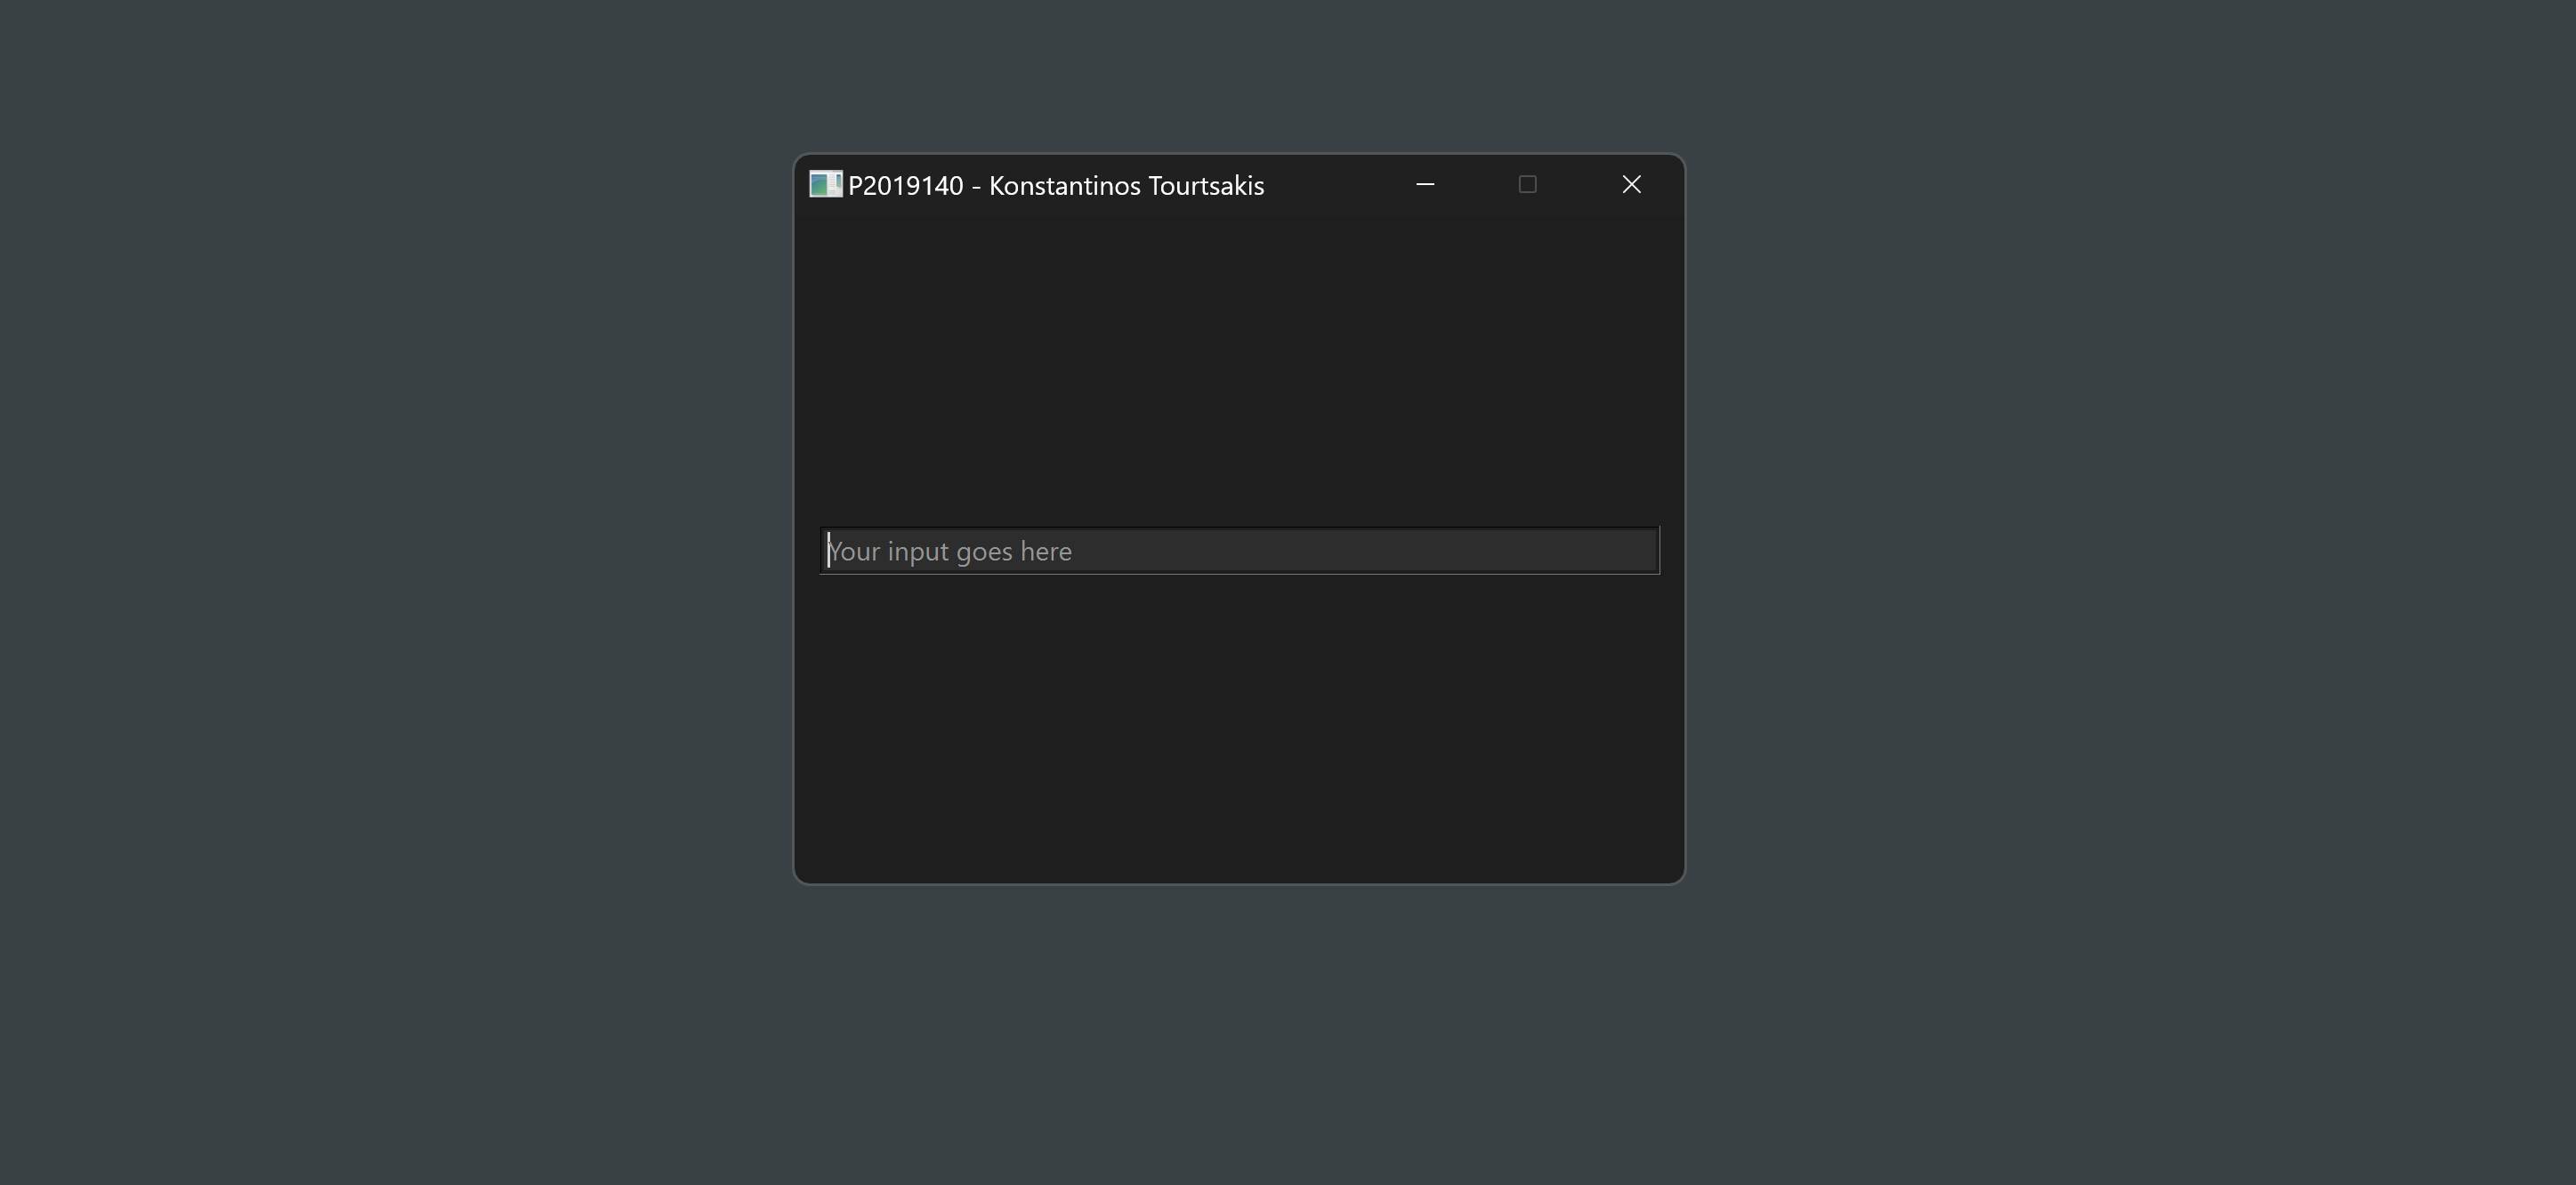
\includegraphics[width=1.0\textwidth]{./images/QLineEdit.png}


\section{Αποθήκευση στοιχείων στον δίσκο}
Κάθε εφαρμογή στις ημέρες μας χρειάζεται να αποθηκεύει την κατάσταση στην οποία
βρισκόταν την τελευταία φορά που εκτελέστηκε με στόχο να γίνει πιο κατανοητή η
χρήση του. Για τον σκοπό αυτό, το Qt φροντίζει να παρέχει τα απαραίτητα εργαλεία
για την αποθήκευση των στοιχείων της εφαρμογής βελτιώνοντας με αυτόν τον τρόπο
τον πηγαίο κώδικα που γράφεται για την προσθήκη της λειτουργίας αυτής. Παρακάτω
βλέπουμε μια μέθοδο που αποθηκεύει τα στοιχεία ενός Qt6 προγράμματος.


\begin{lstlisting}[language=C++, style=cppstyle]
void SaveSettings()
{
    QSettings settings("Company_name", "Application_title");
    settings.beginGroup("group_name");

    settings.setValue("WindowSize", window()->size());
    settings.setValue("Username", "JohnDoe");

    settings.endGroup("group_name");
}

\end{lstlisting}
Αρχικά δημιουργείται ένα αντικείμενο τύπου \textbf{QSettings}. Ακολουθεί ο ορισμός
της ομάδας στην οποία θα γίνουν οι αλλαγές και στην συνέχεια ορίζονται
οι τιμές πάνω στις οποίες θα γραφούν οι μεταβλητές του προγράμματος. Στο τέλος
επαναρχικοποιείται η ομάδα καλόντας την μέθοδο \textbf{endGroup}.

\section{Ανάκτηση εικονιδίων συστήματος αρχείων}
Όπως είναι γνωστό τα γραφικά περιβάλλοντα στηρίζονται πολύ στην χρήση εικονιδίων
για την διευκόλυνση του χρήστη κατά την περιήγησή του μιας και είναι πολύ πιο
αποτελεσματική η συσχέτιση μιας λειτουργίας με μια εικόνα παρά με κάποιο κείμενο.
Επομένως, είναι σημαντικό να υπάρχει μια συνάρτηση που επιστρέφει το εικονίδιο
ενός αρχείου δυναμικά, ώστε ο χρήστης να καταλαβαίνει από την αρχή την λειτουργία που
κρύβεται πίσω από την ενεργοποίηση του εικονιδίου αυτού. Παρακάτω βλέπουμε την συνάρτηση αυτή.


\begin{lstlisting}[language=C++, style=cppstyle]
QIcon GetFileIcon(const QString& file_path)
{
    SHFILEINFO shfi;
    memset(&shfi, 0, sizeof(SHFILEINFO));

    if (SHGetFileInfo(reinterpret_cast<const wchar_t*>(file_path.utf16()), 0, &shfi, sizeof(SHFILEINFO), SHGFI_ICON | SHGFI_USEFILEATTRIBUTES))
    {
        QPixmap pixmap = QPixmap::fromImage(QImage::fromHICON(shfi.hIcon)).scaled(QSize(PercentToWidth(6.66), PercentToHeight(11.85)), Qt::KeepAspectRatio, Qt::SmoothTransformation);
        QIcon icon(pixmap);

        // Cleanup the icon resource
        DestroyIcon(shfi.hIcon);

        return icon;
    }

    
    return QIcon();
}
\end{lstlisting}

Επειδή η εφαρμογή στην οποία αναφέρεται το παρόν κείμενο προορίζεται για χρήση σε
συστήματα Windows, η συγκεκριμένη συνάρτηση στηρίζεται πάνω σε αυτά. Αρχικά
δημιουργείται ένα struct τύπου SHFILEINFO πάνω στο οποίο θα αποθηκευτούν τα
δεδομένα του αρχείου, συμπεριλαμβανομένου και του εικονιδίου. Στην συνέχεια γίνεται
έλεγχος για την ανάκτηση του εικονιδίου από το σύστημα. Αφού η ανάκτηση γίνει με
επιτυχία, δημιουργείται ένα \textbf{QPixmap} με το εικονίδιο του αρχειόυ. Στην 
συνέχεια το pixmap χρησιμοποιείται για την δημιουργία του QIcon εικονιδίου το
οποίο και θα επιστραφεί από την συνάρτηση. Αν το εικονίδιο δεν βρεθεί η συνάρτηση
θα επιστρέψει ένα προεπιλεγμένο QIcon.


\section{Προτάσεις δεδομένων εισόδου σε input field}

Συχνά οι χρήστες βρίσκουν χρήσιμη την υποβοήθησή τους από την γραφική διεπαφή
στην περιήγησή τους στο εκάστοτε πρόγραμμα. Μια τέτοια βοήθεια μπορεί να συμβεί
επίσης στην είσοδο δεδομένων σε ένα input field. Ανάλογα με τις ενέργειες του
χρήστη υπάρχει κάποιος αλγόριθμος που καθορίζει την λίστα από την οποία το
input field θα προτείνει στον χρήστη δεδομένα εισόδου. Στο Qt αυτή η λειτουργία
υλοποιείται με ένα αντικείμενο QCompleter που ουσιαστικά συμπληρώνει αυτό που έχει
γράψει ο χρήστης με προτάσεις δεδομένων.

\begin{lstlisting}[language=C++, style=cppstyle]
    QLineEdit input_field;
    QStringList suggestions;
    suggestions << "Suggestions" << "for" << "thesis";
    
    QCompleter* completer = new QCompleter(suggestions, &input_field);
    completer->setCaseSensitivity(Qt::CaseInsensitive);
    
    input_field.setCompleter(completer);
\end{lstlisting}



\section{Επαναληπτική εκτέλεση διεργασιών παρασκηνίου}

Ένα βασικό πρόβλημα με τις βιβλιοθήκες εφαρμογών γραφικής διεπαφής είναι το γεγονός
πως αμέσως μετά την δημιουργία των γραφικών στοιχείων η βιβλιοθήκη αποκτά τον πλήρη
έλεγχο της εφαρμογής με αποτέλεσμα να μην είναι εφικτή η εκτέλεση κώδικα επαναληπτικά.
Αυτό καθιστά αδύνατη την εκτέλεση διεργασιών ρουτίνας οι οποίες πρέπει να εκτελούνται
σε κάθε επανάληψη του προγράμματος ώστε να γίνει εφικτή η υλοποίηση ορισμένων λειτουργιών.
Ευτυχώς οι περισσότερες βιβλιοθήκες, όπως και το Qt, διαθέτουν αντικείμενα που επιτρέπουν
την προσθήκη κώδικα που εκτελείται σε τακτά χρονικά διαστήματα που ορίζονται από τον
προγραμματιστή. Αυτό όπως είναι κατανοητό μπορεί να αξιοποιηθεί ορίζοντας ένα μηδενικό
χρονικό διάστημα, δημιουργόντας κατά κάποιο τρόπο μια επανάληψη που την διαχειρίζεται το
Qt.

 \begin{lstlisting}[language=C++, style=cppstyle]
QTimer* timer = new QTimer(this);
connect(timer, &QTimer::timeout, this, &MyWidget::TaskMainUserLoop);
timer->start(0);
\end{lstlisting}


\begin{lstlisting}[language=C++, style=cppstyle]
\end{lstlisting}



\chapter{Η βιβλιοθήκη XInput} \label{chapter:xinput}




\section{Τι είναι το XInput;}
Το XInput είναι μια βιβλιοθήκη διαχείρισης εντολών εισόδου για
συσκευές χειρισμού βιντεοπαιχνιδιών κατασκευασμένες από την Microsoft.
Οι συγκεκριμένες συσκευές είναι χειριστήρια Xbox οποιασδήποτε γεννιάς.

\section{Η κλάση του χειριστηρίου}

Για την διαχείρηση των εντολών εισόδου του χειριστηρίου έχει δημιουργηθεί
η αντίστοιχη κλάση. Η κλάση περιλαμβάνει δεδομένα που αφορούν καταστάσεις
του χειριστηρίου, μεθόδους σχετικά με τον έλεγχο καταστάσεων των κουμπιών
του αλλά και μεθόδους που ελέγχουν την συνδεσιμότητα της συσκευής. Παρακάτω
βλέπουμε αναλυτικότερα τον ορισμό της κλάσης και τα στοιχεία που την απαρτίζουν.

\begin{lstlisting}[language=C++, style=cppstyle]
class XBOXController
{
private:
    XINPUT_STATE controller_state;
    int controller_number;
public:
    float left_trigger = 0.0f;
    float right_trigger = 0.0f;

    XBOXController(int playerNumber);
    XINPUT_STATE GetState();
    bool IsConnected();
    void Vibrate(const int left_val = 0, const int right_val = 0);
    SHORT GetLeftAnalogX();
    SHORT GetLeftAnalogY();
    SHORT GetRightAnalogX();
    SHORT GetRightAnalogY();
    bool IsButtonDown(const int button);
    bool IsButtonJustUp(const int button);
    bool IsButtonJustDown(const int button);
};
\end{lstlisting}





\begin{lstlisting}[language=C++, style=cppstyle]
\end{lstlisting}


\chapter{Σχήματα και Πίνακες} \label{chapter:sximata}
\drop{Τ}{Α} 
σχήματα είναι απαραίτητα πολλές φορές για να κατανοήσει
ο αναγνώστης καλύτερα το περιεχόμενο του κειμένου μας.
Μερικές φορές είναι απαραίτητα και για το κείμενό μας.
Επ ουδενί όμως, δεν επιτρέπεται η αντιγραφή (\tl{scan})
σχημάτων άλλων συγγραφέων που υπάρχουν σε βιβλία,
επιστημονικές εργασίες κτλ. 

Όπως τα σχήματα, χρήσιμοι είναι και οι πίνακες 
γιατί μπορεί κάποιος με εύκολο τρόπο να βρει χρήσιμη πληροφορίας,
όπως π.χ. παράθεση πειραματικών αποτελεσμάτων που από τη 
φύση της είναι δύσκολη και ίσως δυσνόητη όταν 
βρίσκεται εντός του κειμένου.

\section{Σχήματα}

Στη συνέχεια θα δωθούν μερικά παραδείγμα μορφής σχημάτων.

Το ``κλασικό'' σχήμα είναι αυτό που
απεικονίζεται στο Σχήμα \ref{fig:intro_data_flow}.
Προφανώς, το σχήμα μπορεί να θέλει να είναι λίγο μικρότερο
(π.χ., όπως στο Σχήμα \ref{fig:intro_data_flow2})
αλλά φροντίζουμε να μην είναι το πλάτος του μικρότερο από
το 1/2 του πλάτους του κειμένου. Σε κάθε περίπτωση, 
τα σχήματα αριθμούνται ξεχωριστά για κάθε κεφάλαιο
αρχίζοντας από το 1 με πρόθεμα το νούμερο του κεφαλαίου.

\myfig{intro_data_flow}
{Ένα δίκτυο.}

\myfigadapt{intro_data_flow2}
{To ίδιο δίκτυο  που
απεικονίζεται στο Σχήμα \ref{fig:intro_data_flow}
αλλά λίγο μικρότερο.
}
{0.5}




Υπάρχουν περιπτώσεις που μπορεί κάποιος να
θέλει δύο ίδια σχήματα δίπλα-δίπλα,
όπως είναι η περίπτωση του Σχήματος \ref{fig:intro_data_flow3}.
Προφανώς μπορεί να γίνει ξεχωριστή αναφορά στα
δύο υπο-σχήματα \ref{fig:intro_data_flow}.α και \ref{fig:intro_data_flow}.β
με τον αυτό τρόπο.
Το κείμενο για τα δύο υποσχήματα είναι προαιρετικό αλλά η αρίθμηση υποχρεωτική.

\mytfig{intro_data_flow3}
{Το ίδιο δίκτυο σε διπλή απεικόνιση.}
{Κείμενο για το πρώτο.}
{Κείμενο για το δεύτερο.}

Όπως προηγουμένως, μπορεί να είναι επιθυμητή
η αλλαγή του μεγέθους των σχημάτων, όπως φαίνεται στο 
Σχήμα \ref{fig:intro_data_flow4}.


\mytfigadapt{intro_data_flow4}
{Το ίδιο δίκτυο σε διπλή απεικόνιση σε σμίκρυνση
και δίχως κείμενο για τα υπο-σχήματα.}
{}
{}
{0.3}
{0.3}


Τέλος, υπάρχει το ενδεχόμενο να είναι αναγκαία 
η παρουσίαση κάποιων σχημάτων σε τετράδα,
όπως είναι το Σχήμα \ref{fig:intro_data_flow5}.

\myffig{intro_data_flow5}
{Το ίδιο δίκτυο σε τετραπλή απεικόνιση.}
{Κείμενο για το πρώτο.}
{Κείμενο για το δεύτερο.}
{Κείμενο για το τρίτο.}
{Κείμενο για το τέταρτο.}

Με όμοιο τρόπο όπως προηγουμένως μπορεί να επιτευχθεί
αλλαγή του μεγέθους.


\section{Πίνακες}

Οι πίνακες ομοιάζουν με το κλασικό σχήμα στη μορφή και
την αναφορά σε αυτούς, με μόνη διαφορά πως προηγούνται αντί να έπονται,
όπως φαίνεται και στο παράδειγμα του Πίνακα \ref{tbl:example}.

%table
\begin{table}
\caption{Παράδειγμα Πίνακα.}
\label{tbl:example}
\begin{center}
\begin{tabular}{|p{18mm}|p{12mm}|p{12mm}|p{12mm}|p{12mm}|p{12mm}|p{12mm}|p{12mm}|}\hline
		& 	$s_0$&	$s_1$& $s_2$	& $s_3$	& $s_4$	& $s_5$	& $s_6$	\\ \cline{1-8}
$f_0(s_\chi)$	& 	$1$	&	$2$	& $3$	& $4$	& $5$	& $6$	& $0$	\\ \cline{1-8}
$f_1(s_\chi)$	&	$1$	&	$3$	& $5$	& $0$	& $2$	& $4$	& $6$	\\ \cline{1-8}
$f_2(s_\chi)$	&	$4$	&	$0$	& $3$	& $6$	& $2$	& $5$	& $1$	\\ \cline{1-8}
$f_3(s_\chi)$	&	$3$	&	$0$	& $4$	& $1$	& $5$	& $2$	& $6$	\\ \cline{1-8}
$f_4(s_\chi)$	&	$2$	&	$5$	& $1$	& $4$	& $0$	& $3$	& $6$	\\ \cline{1-8}
$f_5(s_\chi)$	&	$2$	&	$3$	& $4$	& $5$	& $6$	& $0$	& $1$	\\ \cline{1-8}
$f_6(s_\chi)$	&	$6$	&	$4$	& $2$	& $0$	& $5$	& $3$	& $1$	\\ \cline{1-8}
$f_7(s_\chi)$	&	$1$	&	$0$	& $6$	& $5$	& $4$	& $3$	& $2$	\\ \cline{1-8}
$f_8(s_\chi)$	&	$5$	&	$6$	& $0$	& $1$	& $2$	& $3$	& $4$	\\ \cline{1-8}
$f_9(s_\chi)$	&	$3$	&	$2$	& $1$	& $0$	& $6$	& $5$	& $4$	\\ \hline
\end{tabular}
\end{center}
\end{table}



\chapter{Τελευταία Μέρη} \label{chapter:telos}
\drop{Έ}
χοντας πλέον μελετήσει το πρόγραμμα αυτό και αποκτήσει μια καλή κατανόηση του
προβλήματος που προσπαθεί να λύσει, μπορούμε πια να δούμε καλύτερα πώς μπορεί
να είναι χρήσιμο στη δική μας χρήση του Η/Υ. Η υλοποίηση αυτού του προγράμματος
αποτελεί όχι απλώς ένα παράδειγμα μιας ακόμη εφαρμογής εκτέλεσης προγραμμάτων αλλά
παρουσιάζει και τα μειονεκτήματα των σύγχρονων γραφικών περιβαλλόντων που χρησιμοποιούν
τα δημοφιλή για οικιακή χρήση λειτουργικά συστήματα. Η εκτέλεση ενός προγράμματος
και η περιήγηση στο σύστημα αλλά και το ίδιο το πρόγραμμα είναι ένα σημαντικός παράγοντας
που καθορίζει την επιλογή του χρήστη ενός προσωπικού υπολογιστή. Οι εναλλακτικές λύσεις που
υπάρχουν για την πρόσβαση σε λογισμικό με τις επιπρόσθετες περιφερειακές συσκευές
θέτουν τον χρήστη σε ένα περιβάλλον που περιορίζει τις δυνατότητές του λόγω της έλλειψης
σημαντικών desktop εφαρμογών ή της υπολογιστικής ισχύος που απαιτείται για την εκτέλεσή τους.
Όσον αφορά τις τεχνολογίες που χρησιμοποιήθηκαν για την υλοποίηση του προγράμματος αυτού:
\begin{itemize}
	\item
Το Qt είναι ένα εξαιρετικό εργαλείο για τη δημιουργία εφαρμογών γραφικής διεπαφής. Προσφέρει
μια μεγάλη ποικιλία γραφικών στοιχείων που μπορούν να τροποποιηθούν για τις ανάγκες της εκάστοτε
εφαρμογής. Είναι αρκετά απλό και είναι επαρκές για την υλοποίηση πρακτικά κάθε λειτουργίας της
εφαρμογής. Επιπλέον, ως μια cross-platform βιβλιοθήκη αποτελεί μια καλή λύση που έχει την ευελιξία
να λειτουργήσει σε πολλαπλά συστήματα που υποστηρίζει.
	\item
Το XInput προσφέρει μια αρκετά κατανοητή λύση στην διαχείριση εισόδου από ένα χειριστήριο βιντεοπαιχνιδιών
τύπου Xbox και έπαιξε σημαντικό ρόλο στην επίτευξη του στόχου της εφαρμογής αυτής.
	\item
Το Windows είναι το λειτουργικό σύστημα που φιλοξένησε την εφαρμογή. Αρκετές λειτουργίες της βασίζονται πάνω
σε αυτό και ως το δημοφιλέστερο λειτουργικό σύστημα προσωπικού υπολογιστή αποτελεί ένα καλό παράδειγμα πάνω
στο οποίο παρουσιάστηκε η λύση του προβλήματος αυτού.
\end{itemize} 

 




%CHAPTER
\chapter*{Παράρτημα Α'} \pagestyle{empty}
\addcontentsline{toc}{chapter}{Παράρτημα Α'}
Ενδεικτικό παράδειγμα παραρτήματος.
Έπεται το κεφάλαιο της βιβλιογραφίας.



%Bibliography
\begin{thebibliography}{99} \addcontentsline{toc}{chapter}{Βιβλιογραφία}
\pagestyle{headings}
\bibitem{example}
\tl{Authors,
\textit{title}, information about the book, paper journal.}

\end{thebibliography}


%CHAPTER
\chapter*{Συντμήσεις} \pagestyle{empty}
\addcontentsline{toc}{chapter}{Συντμήσεις}




\gl
{\tl{DNS}}
{\tl{Domain Name Server}}





%CHAPTER
\chapter*{Γλωσσάρι Ξενικών Όρων} \pagestyle{empty}
\addcontentsline{toc}{chapter}{Γλωσσάρι Ξενικών Όρων}
%\Huge{\tl{A}}
%\normalsize

\gl
{\tl{Access Permissions}}
{Δικαιώματα Πρόσβασης}
\gl
{\tl{Adapter}}
{Προσαρμογέας}
\gl
{\tl{Administrator}}
{Επιβλέπων}
\gl
{\tl{Agent}}
{Πράκτορας}


\gl
{\tl{Background Process}}
{Διεργασία Παρασκηνίου}



\gl
{\tl{Capture}}
{Καταγράφω}
\gl
{\tl{Capture Filter}}
{Φίλτρο Καταγραφής}
\gl
{\tl{Command Mode}}
{Κατάσταση Εντολών}
\gl
{\tl{Configuration}}
{Καθορισμός Παραμέτρων}
\gl
{\tl{Configuration Files}}
{Αρχεία Παραμέτρων}
\gl
{\tl{Connector}}
{Σύνδεσμος}
\gl
{\tl{Console Port}}
{Θύρα Κονσόλας}
\gl
{\tl{Crossover Cable}}
{Διασταυρωμένο Καλώδιο}


\gl
{\tl{Demodulation}}
{Αποδιαμόρφωση}
\gl
{\tl{Desktop}}
{Επιφάνεια Εργασίας}
\gl
{\tl{Device Files}}
{Αρχεία Συσκευών}
\gl
{\tl{Display Filter}}
{Φίλτρο Προβολής}
\gl
{\tl{Driver}}
{Πρόγραμμα Οδήγησης}
\gl
{\tl{Download}}
{Κατέβασμα Αρχείων}


\gl
{\tl{Foreground Process}}
{Διεργασία Προσκηνίου}
\gl
{\tl{Forwarding}}
{Προώθηση}


\gl
{\tl{Header}}
{Κεφαλίδα}
\gl
{\tl{Hub}}
{Συζεύκτης}

\gl
{\tl{Internet Lab}}
{Εργαστήριο Διαδικτύου}
\gl
{\tl{Internet Lab Manual}}
{Εγχειρίδιο του Εργαστηρίου Διαδικτύου}

\gl
{\tl{Kernel}}
{Πυρήνας}

\gl
{\tl{Modem}}
{Διαμορφωτής-Αποδιαμορφωτής}
\gl
{\tl{Modulation}}
{Διαμόρφωση}
\gl
{\tl{Mount}}
{Αγκίστρωση Συστήματος Αρχείων}


\gl
{\tl{Network Interface}}
{Διεπαφή Δικτύου}
\gl
{\tl{Network Protocol Analyzers}}
{Αναλυτές Δικτυακών Πρωτοκόλλων}


\gl
{\tl{Overwrite}}
{Επανεγγραφή}



\gl
{\tl{Packet Sniffer}}
{Συλλέκτης Πακέτων}
\gl
{\tl{Pathname}}
{Μονοπάτι}
\gl
{\tl{Physical Layer}}
{Φυσικό Επίπεδο}
\gl
{\tl{Pin}}
{Απόληξη}
\gl
{\tl{Prompt}}
{Χαρακτήρα Εισόδου Εντολών}


\gl
{\tl{Rebooting}}
{Επανεκκίνηση}
\gl
{\tl{Rollover Cable}}
{Ανεστραμμένο Καλώδιο}
\gl
{\tl{Router}}
{Δρομολογητής}




\gl
{\tl{Shell}}
{Φλοιός}
\gl
{\tl{Straight-through Cable}}
{Απευθείας Καλώδιο}


\gl
{\tl{Upload}}
{Ανέβασμα Αρχείων}


\gl
{\tl{Window Manager}}
{Διαχειριστής Παραθύρων}






\newpage
\addcontentsline{toc}{chapter}{Ευρετήριο}
\printindex



\end{document}
